% Chapter Template
\tocdata{toc}{Edward Gunn}

\chapter{Model} % Main chapter title

\label{Chapter4} % Change X to a consecutive number; for referencing this chapter elsewhere, use \ref{ChapterX}

%----------------------------------------------------------------------------------------

% Define some commands to keep the formatting separated from the content 
\newcommand{\keyword}[1]{\textbf{#1}}
\newcommand{\tabhead}[1]{\textbf{#1}}
\newcommand{\code}[1]{\texttt{#1}}
\newcommand{\file}[1]{\texttt{\bfseries#1}}
\newcommand{\option}[1]{\texttt{\itshape#1}}

%----------------------------------------------------------------------------------------

%----------------------------------------------------------------------------------------
%	SECTION 1
%----------------------------------------------------------------------------------------

\section{Introduction}


The problem of generation of a set of chords from a melody is very similar to that of translating one language to another. 
The translation problem is one that is very popular in machine learning research and thus there are many resources on it.  
However, the music related problem is harder to solve due to the extra dimension each of its elements contains. 
Each element in a melody has both pitch, represented by a discrete symbol or note, and duration whereas each element in the sequence of language is composed of only the discrete symbols or words.  
Therefore, in order to use techniques developed for natural language processing, it is necessary to encode the melody and chords in such a way that their dimensions are collapsed into one. 
Since this collapsing of dimensions has already been conducted in \autoref{Chapter3} we are able to take full advantages of NLP techniques.
There have been many attempts to apply some of these techniques to the chord generation problem. 
In order to find the best model we evaluate these attempts against defined criteria and develop a novel model to evaluate against the same criteria.


\section{Model Requirements}
\label{sec:Evaluation}
\subsection{MVP Requirements}
\label{sec:MVPRequirements}
The MVP requirements were defined at the beginning of the project to ensure it is compatible with the other parts of the product that were simultaneously in development and to ensure the possibility of the creation of the prototype for proof of concept. 
We required the model to be a black box in which we could input a melody, and it would output chords which sounded good.
The notion of sounding good is intentionally vague as what sounds good or bad is usually down to individual taste in music.
There is never a definitive answer to which chords would sound the best.
However, we felt that even people without any musical training would be able to judge whether chords fit the melody relatively accurately.
This is supported by the finding that musical training is not required to respond to music is sophisticated ways in \cite{ExperiencedListeners}.
Within this overarching requirement we defined tighter constraints for the sake of both practicality and user experience. 
The model would have to be designed for sequential data such that the temporal relationship of the different notes being played were taken into account.
It would be possible to simply learn a function where, for a given measure, a chord suited to the notes played within that measure was generated without taking into account surrounding measures.
This approach could produce reasonable results and be significantly more simple that other options, however, the quality and variation of chords generated would be lower than that of a model for sequential data, hence our choice to forego it.
The model would also have to be conditional. For a given input it should produce a catered output. This is an obvious constraint however for models such as a GAN it requires changes to the format of the input data.
To maximise user experience the models should be non-deterministic. This allows users to regenerate the accompaniment multiple times to obtain new chords and thus means they can choose what they feel is best.
For practicality's sake we constrained our MVP to only require one chord to be played each measure as the problem of determining when a chord should be played is of similar difficulty to choosing which chord to play.
\subsection{Other possible Requirements}

There were some constraints which were not used in our project which would provide better quality chords, but this provided too large a practical barrier to be implemented.
The act of collapsing the pitch and duration of the notes into a single dimension removes information from the melody.
In our case this information is the order in which the notes are played and the rhythmic intention of the composer.
It is likely a model would be able to produce more suitable chords given this information.
Thus, for a stricter set of constraints we could include the requirement that the order and duration of notes are both maintained in the data.
The accompaniment for music is not limited to a single chord played at the start of each bar.
A much more interesting accompaniment would be generated if it were not limited to this restrictive format.
As shown in \cite{ReinforcementLearning} it is possible to create a model which learns the divisions within the music and thus learns when it would be most appropriate to play a chord.
Therefore, in order to allow for more interesting accompaniment, the requirement of one chord per bar could be changed such that chords are played with closer freedom to that of a human composer.
% Strongly temporal

\subsection{Evaluation criteria}
\paragraph{Approach}
Many attempts to solve the chord generation problem have been made each of which contain variants on models and implementations which result in large variations in metrics used for evaluation.
There is also a large variation in features for which quantative evaluation is impossible. 
As it would be impractical to implement each relevant model ourselves to allow for full standardisation of evaluation, we will evaluate models built ourselves and from previous work based on a set of criteria defined below.
\paragraph{Data}
One of the biggest influences on the effectiveness of a model is the dataset on which it is trained. 
In general a larger dataset results in a better generalisation of learning \cite{UnreasonableEffectivenessOfData}.
Most datasets are comprised of lead sheets which can be translated into chord melody pairs.
Many datasets are then further divided down into measures in which there is one chord played per measure and the melody within that measure is somehow encoded.
Thus, for best comparison the number of measures used in the dataset is a good criterion for evaluation.
This is a particularly important area for evaluation as it will strongly affect the output of the model and thus the results of other 

\paragraph{Quantitative Evaluation}
There is difficulty in quantative evaluation for this problem as there is no strictly correct chords for a given melody and thus comparison to any specific set of chords gives a skewed interpretation of the output.
However, the use of conventional quantative evaluation does still correlate strongly with the sentiment given by a human judging the quality of chords and thus can be cautiously used in evaluation.
The test set from the data can be used to compare the outputs from the model to previously assigned chords. Accuracy can be found by finding the number of chords successfully predicted and dividing by the total number of chords produced.
\begin{equation}
    \text{Accuracy} = \frac{\text{Number of Chords Correctly Assigned}}{\text{Total Number of Chords Generated}}
\end{equation}
As this was the only quantative measure consistently used across previous implementations this is the only one we will consider for evaluation.

\paragraph{Qualitative Evaluation}
Some previous work \cite{MySong}, \cite{BLSTM} carried out experiments to judge the sentiment of untrained musicians to the generated chords.
Participants were played the melody accompanied by a varying set of chords and asked to judge which chords they felt were best out of a set containing chords generated by models and some human written accompaniment.
The results from these experiments can be used to compare models to each other as well as evaluate them relative to the standard set by human written chords.
As well as evaluation based on the quality of chords produced we will discuss extra functionality made possible by some models and the effect this has on other evaluation metrics.

\paragraph{Criteria}
The final criteria used for evaluation are thus:
\begin{itemize}
    \item Number of measures in the dataset
    \item Accuracy in testing
    \item Human sentiment towards generated chords
    \item Extra functionality the model provides
\end{itemize}
\section{Models}

We now apply this evaluation criteria to a number of models suited to solving the chord generation problem. 
Specifically we explore the implementations of models from other papers before discussing how a transformer could be implemented to solve this problem.

\subsection{HMMs}
\label{subsec:HMM}
\subsubsection{Explanation and Applicability}
Hidden Markov Models or HMMs were first put forward by Leonard E. Baum in a series of statistical papers \cite{HMM1} \cite{HMM2} \cite{HMM3}. 
They model a stochastic process in which the desired states, $\boldsymbol{X}$, are not directly observable but related states, $\boldsymbol{Y}$, which directly influence the desired states are. 
By modelling the $\boldsymbol{X}$ and $\boldsymbol{Y}$ as Markov Processes 
we are able to infer the hidden state.
To apply an HMM to our problem we take the hidden state, $\boldsymbol{X}$, to be the chords played, and the observable state $\boldsymbol{Y}$ to be the Melody.
It is notable that the conditional probability distribution of the hidden variable $x(t)$ at time t, only depends on that of the previous time step $x(t-1)$ and that $y(t)$ only depends on the hidden distribution at the current time step $x(t)$.
For our purposes this limits the "memory" the model could have to a single measure and thus seriously reduces the effect of relationship between chords across time.

\subsubsection{Implementations}

\paragraph{MySong} The first application of an HMM to this problem whilst also being the first attempt focusing specifically on a vocal melody from \cite{MySong} used an Augmented Hidden Markov Model with parameters such that users could adjust the "Happy Factor" and "Jazz Factor" to alter the mood of the generated chords to their preference.
No measure was given for the accuracy of the model, however a study which compared the quality of MySong to manually assigned chords was carried out. 
In 264 comparisons the participants preferred MySong 95 times, manual 121 times and had no preference 48 times
The additional user input possible with the "Happy factor" and "Jazz factor" parameters are reported to significantly improve the user experience, however, this is their only implementation and so nothing can be inferred about the quality of the HMM itself.

\paragraph{Chord Generation from Symbolic Melody}  As a comparison for the main model in \cite{BLSTM} an HMM was implemented. 
The HMM is trained on a reduced version of the 
wikifonia.org\footnote{Wikifonia shut down in 2013, but the dataset is still available from http://marg.snu.ac.kr/chord\_generation/ for academic purposes} dataset which includes an array of Western music genres with 2,252 lead sheets, 1802 of which are used for training. 
This overall comes to 72,418 measures for the training set and 17,768 for the test set. 
They tested the accuracy of the HMM on sequences of length 4, 8, 12, and 16 bars long, gaining an accuracy of $0.4033$, $0.4043$, $0.4041$, and $0.4045$ respectively and an average accuracy of $0.4041$.
They also carried out a user subjective test with 25 participants each evaluating 18 sets, each set containing a melody accompanied by three generated chord sequences and an original chord sequence.
The users would listen to the music played and judge the accompaniment on a scale of 1, being not appropriate, and 5, being very appropriate.
The HMM achieved an average score of $2.31$ and the original chords achieved an average score of $4.04$.

\paragraph{Machine Learning in Automatic Music Chords Generation} An HMM was tested in \cite{MLForChords} along with other simpler models. It was trained on 43 lead sheets, with 813 measures total. 
An accuracy of $0.4844$ was achieved, however, a choice of only 7 chords were used unlike the usual 24.

% \paragraph{Autoarrangement System of Accompaniment Chords} An HMM with improved PCP feature extraction was used in \cite{HMMswithML} 

\subsection{DNN-HMMs}

\label{subsec:DNN-HMMs}
\subsubsection{Explanation and Applicability} 

A deep neural network HMM makes it possible to assume a posterior for the HMM using the output from the softmax output layer of the DNN. 
This allows for the posterior to be learned in training.

\subsubsection{Implementations}

\paragraph{Chord Generation from Symbolic Melody} This was implemented much like the HMM from \cite{BLSTM} mentioned above in \autoref{subsec:HMM}.
The same dataset was used and an accuracy of $0.4502$, $0.4482$, $0.4495$, and $0.4468$  was obtained on the 4, 8, 12 and 16 bars respectively. This results in an average accuracy of $0.4487$.
On the user subjective test the DNN-HMM achieved a score of $2.48$.

\subsection{GANs}

\subsubsection{Explanation and Applicability}

Generative Adversarial Networks or GANs were first proposed in the landmark paper \cite{GANs}. Unlike most models GANs consist of two separate agents working against each other.
The first model, the Generator, takes an input of random noise and outputs data which mimics the training data. 
The second model, the Discriminator, takes as input an example from the training data or an output from the Generator and outputs a value between 0 and 1 indicating whether it thinks the input is real or generated.
The Binary Cross Entropy loss is used for the Discriminator averaged across real and generate examples. The loss for the Generator is the log complement of that for the Discriminator. Thus, the two models play the following minmax game:
\begin{equation}
\underset{D}{\text{min}} \underset{G}{\text{max}} V(D,G) = \mathbf{E}_{x\sim p_{data}(\mathbf{x})}[logD(\mathbf{x})] + \mathbf{E}_{z\sim p_{data}(\mathbf{z})}[log(1-D(G(\mathbf{z})))]
\end{equation} 
Theoretically the Generator and Discriminator can be any differentiable function thus leaving much room for flexibility.
The problem with GANs for our uses is that they are not conditional, the only input to the Generator is noise. A proposed remedy for this was presented in \cite{CGANs}.
By concatenating the label data, in our case the melody, with the noise as input to the Generator and doing the same with the training data and the label data, in our case a chord and melody, as input to the Discriminator GANs can be made conditional. 
Thus, they would be suitable for our uses. 

\subsubsection{Implementations}

\paragraph{ChordGAN} \cite{ChordGAN} uses a conditional GAN along with Chroma Feature Extraction to generate chords for a specific genre of music based on the dataset it was trained on.
They used three different data sets one for each Pop, Jazz and Classical music each shorter than 1600 measures (specific lengths are not given).
The model achieved an accuracy of $0.68$, $0.74$ and $0.64$ respectively across the datasets.

\subsection{RNNs}

Recurrent Neural Networks or RNNs have become a staple in the machine learning engineer's library of models. 
They are structured much like a normal MLP, however, they contain an extra connection to the state of the network in the time step before.
This means that the state of the network at each time step depends on that of the previous time step and thus the state at the current time step is affected by the state in all previous time steps.
This makes RNNs ideal for processing sequential data as temporal relationships are taken into account.
The gradient of RNNs can be found using a variation of the backpropagation algorithm usually know as backpropagation through time.
RNNs that operate on large sequences often experience the problems of exploding or vanishing gradients leading to a saturation of learning.

\begin{figure}
    \centering
    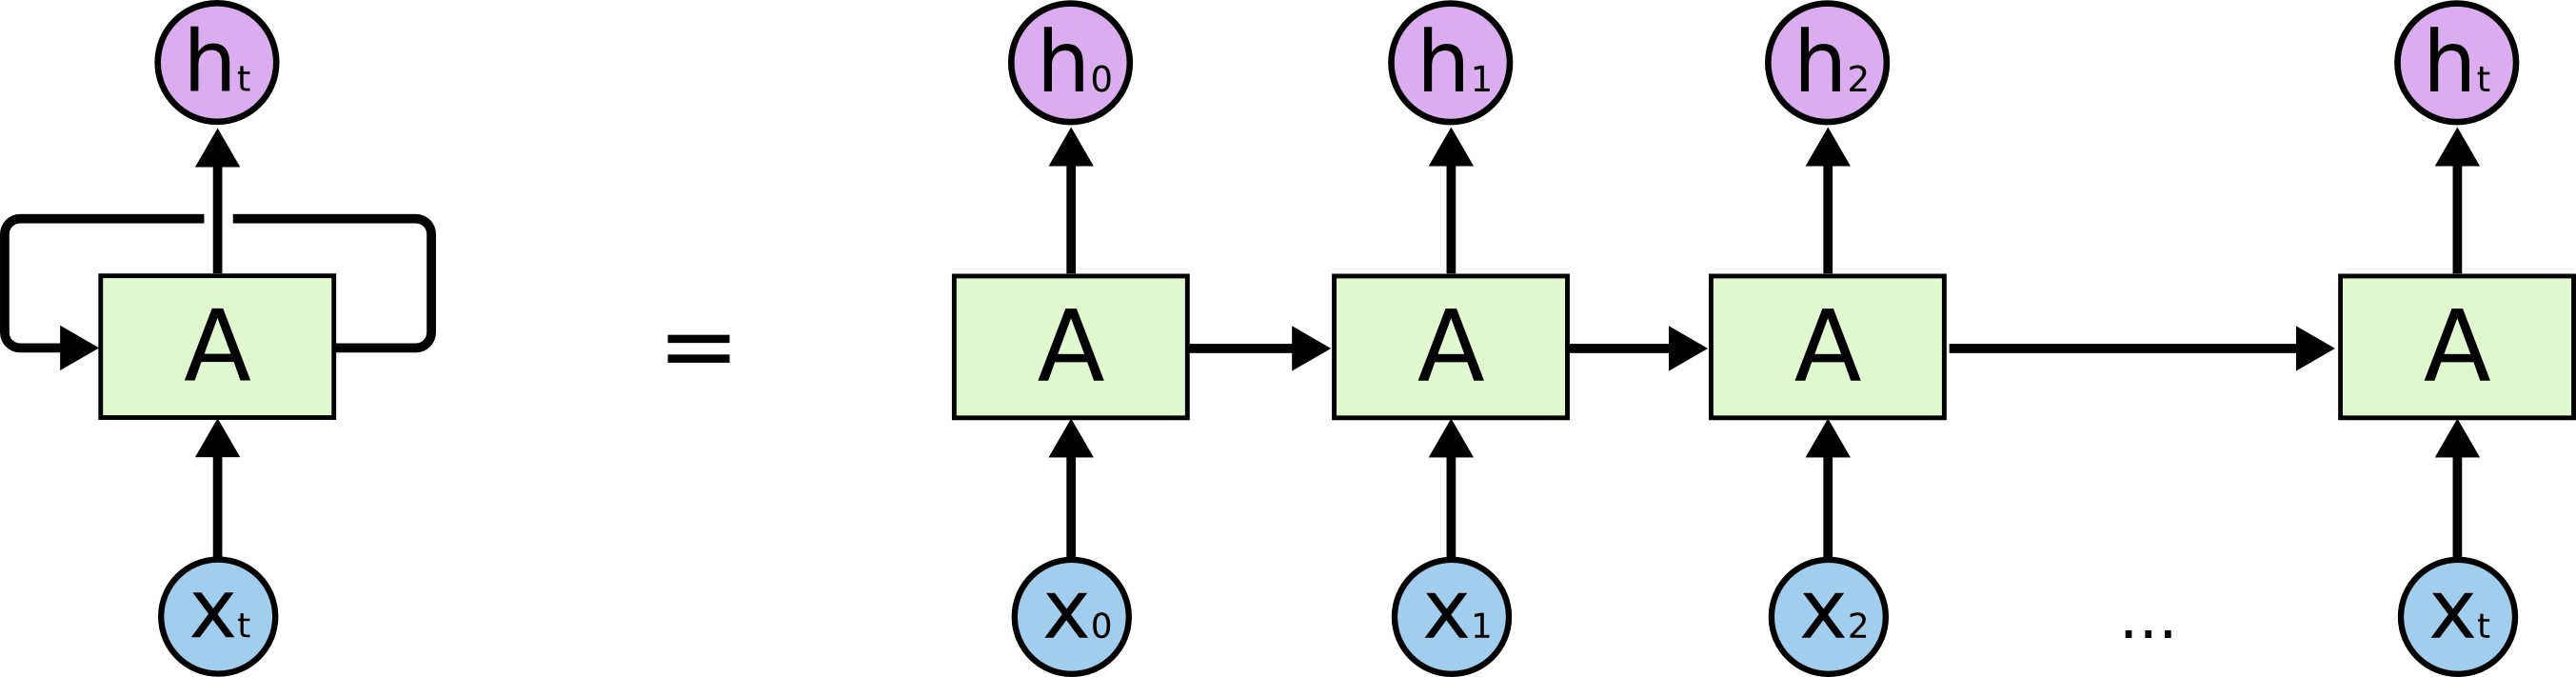
\includegraphics[width=0.8\columnwidth]{Figures/RNN}
    \decoRule
    \caption[An RNN]{A many inputs to many outputs diagram of an RNN from \cite{oinkina}}
    \label{fig:RNN}
\end{figure}

\subsection{LSTMs}

The Long Short Term Memory model or LSTM was proposed in \cite{LSTMs} in order to overcome the gradient problems related to RNNs and thus allow for faster training on long sequences.
They are also capable of learning longer dependencies due to their internal memory. An LSTM cell has three gates: input, forget, and output.
The state of these gates determines whether the cell allows new input, forgets old information, and affects the output at the current time step.
At time step t, the states of the gates are given by:
\begin{equation}
    i_t=\sigma(w_i[h_{t-1},x_t]+b_i)
\end{equation}
\begin{equation}
    f_t=\sigma(w_f[h_{t-1},x_t]+b_f)
\end{equation}
\begin{equation}
    o_t=\sigma(w_o[h_{t-1},x_t]+b_o)
\end{equation}
where $i_t$, $f_t$ and $o_t$ denote the input, forget, and output gates state respectively, $h_{t-1}$ is the output at the previous time step.
$w$ and $b$ represent weights and biases of each gate, $x_t$ is the input to the LSTM cell, and $\sigma (.)$ is the sigmoid function applied elementwise.
The current output of the cell is computed by:
\begin{equation}
    h_t=o_t \circ tanh(c_t)
\end{equation}
\begin{equation}
    c_t = f_t \circ c_{t-1}+i_t \circ \overset{\sim}{c}_t
\end{equation}
\begin{equation}
    \overset{\sim}{c}_t = tanh(w_c[h_t,x_t]+b_c)
\end{equation}

\begin{figure}
    \centering
    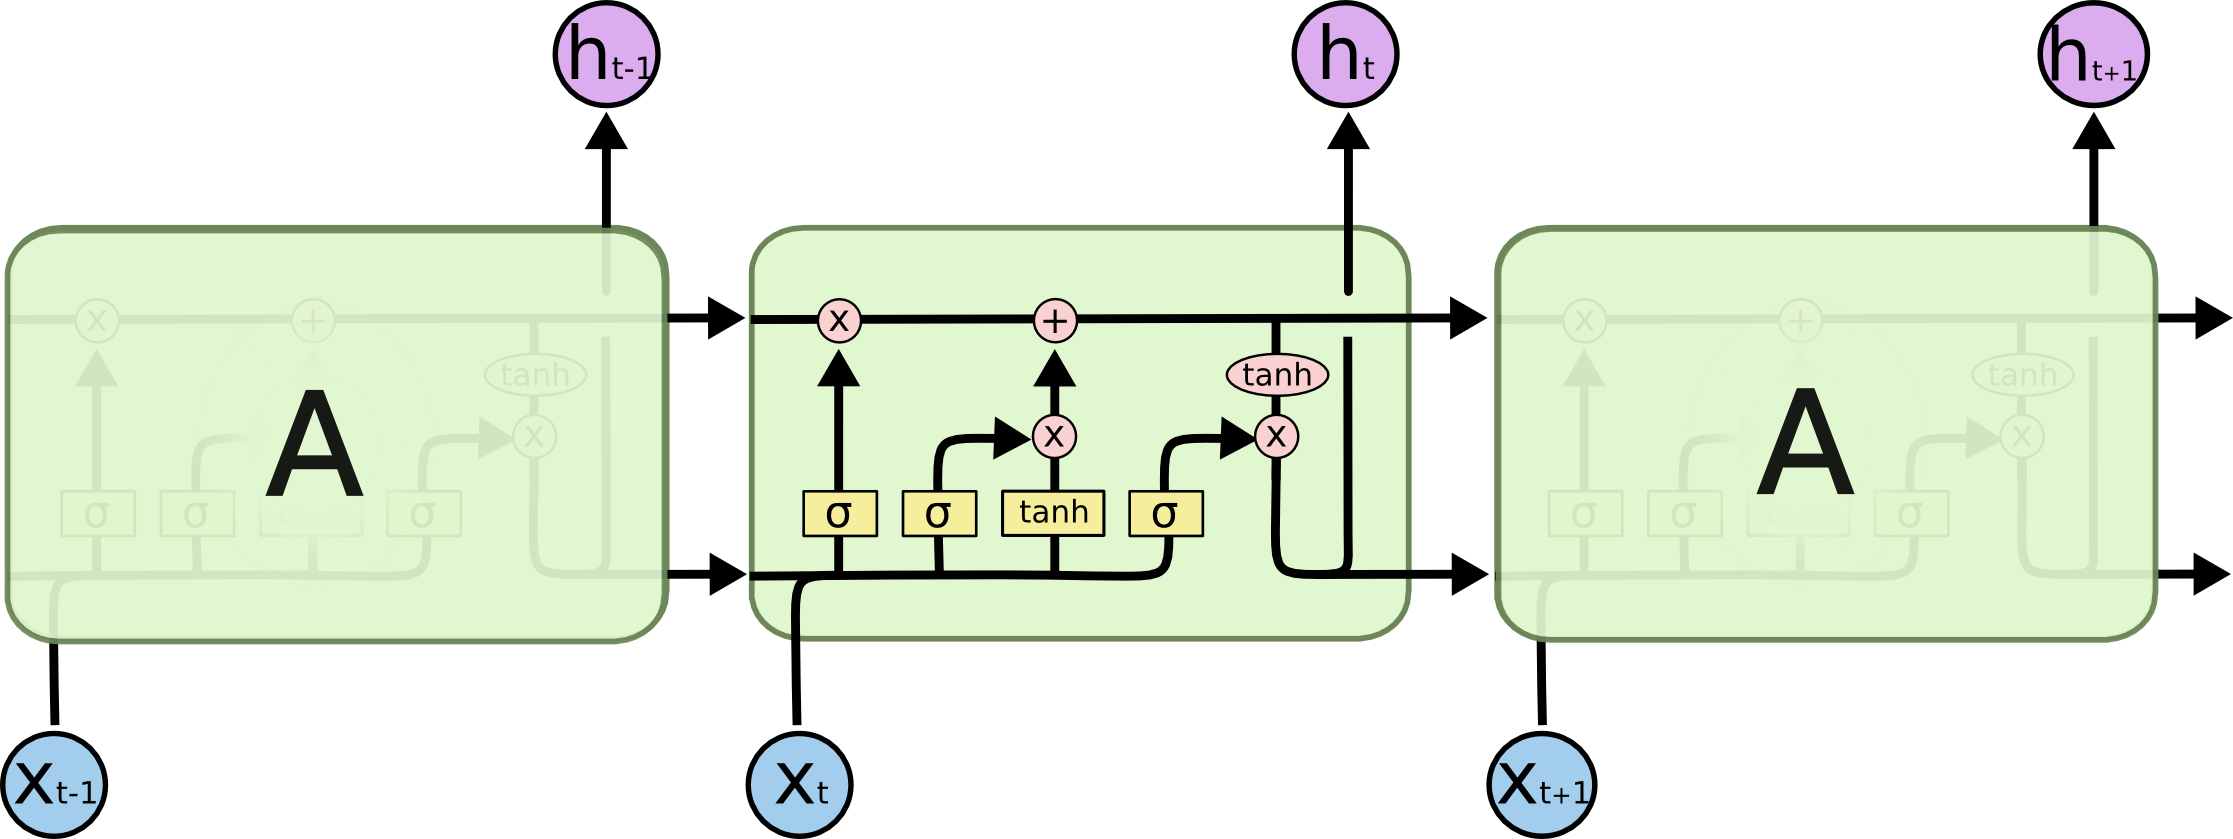
\includegraphics[width=0.8\columnwidth]{Figures/LSTM}
    \decoRule
    \caption{The repeating module in an LSTM from \cite{oinkina}}
    \label{fig:LSTM}
\end{figure}

\subsubsection{Implementations}

\paragraph{Chord Generation from Symbolic Melody} This was the main model under scrutiny in \cite{BLSTM} mentioned above in \autoref{subsec:HMM} and \autoref{subsec:DNN-HMMs}.
They build a bidirectional LSTM with two hidden layers and used a hyperbolic tangent activation function. The softmax function is applied to the output in order to represent the probability that each of the 24 chords is played.
The same dataset as the HMM and DNN-HMM was used and an accuracy of $0.5055$, $0.5032$, $0.4923$, and $0.4990$  was obtained on the 4, 8, 12 and 16 bars respectively. This results in an average accuracy of $0.5000$.
On the user subjective test the DNN-HMM achieved a score of $3.55$.

\paragraph{Automatic Melody Harmonization} A particularly interesting model heavily relying on LSTMs surrounded by a reinforcement learning framework was proposed in \cite{ReinforcementLearning}.
They simultaneously trained a Structured Representation Module responsible for learning note-level, phrase-level and segment level representations, a Segmentation Module acting as a reinforcement learning agent to decide whether the current note is the boundary of a phrase or segment and a Harmonisation Module responsible for generating chords for each segment.
They used the Hooktheory Lead Sheet Dataset with 10,000 songs, no number of measures is given but with the difference in model architecture so drastic a comparison on this metric would be inappropriate anyway.
The achieved an accuracy of $0.3742$ and compared that to an SVM, CNN, LSTM and BLSTM with blocked Gibbs sampling which achieved an accuracy of $0.2516$, $0.2664$, $0.2802$, $0.2933$ respectively.
% The inclusion of variable numbers of chords in each measure greatly expands the possibilities with music composition

\subsection{Transformers}
\label{Transformers Ed}
\subsubsection{Explanation and Applicability}

Transformers have been a revolutionary development in the field of NLP, first proposed by \cite{Transformers} they have become very widely used and regularly produce state-of-the-art performance.
Transformers utilise the encoder decoder model for sequence to sequence translation.
They also heavily use attention which is a mechanism for weighting the importance of different elements of a sequence of data.
Specifically they propose the Scaled dot-product attention shown in \autoref{eq:Attention}
\begin{equation}
    \text{Attention}(Q,K,V) = \text{softmax}(\frac{QK^T}{\sqrt{d_k}})V
    \label{eq:Attention}
\end{equation}
where $Q$, $K$ and $V$ represent the queries, keys and values respectively and $d_k$ is the dimension of queries and keys.

\begin{figure}
    \centering
    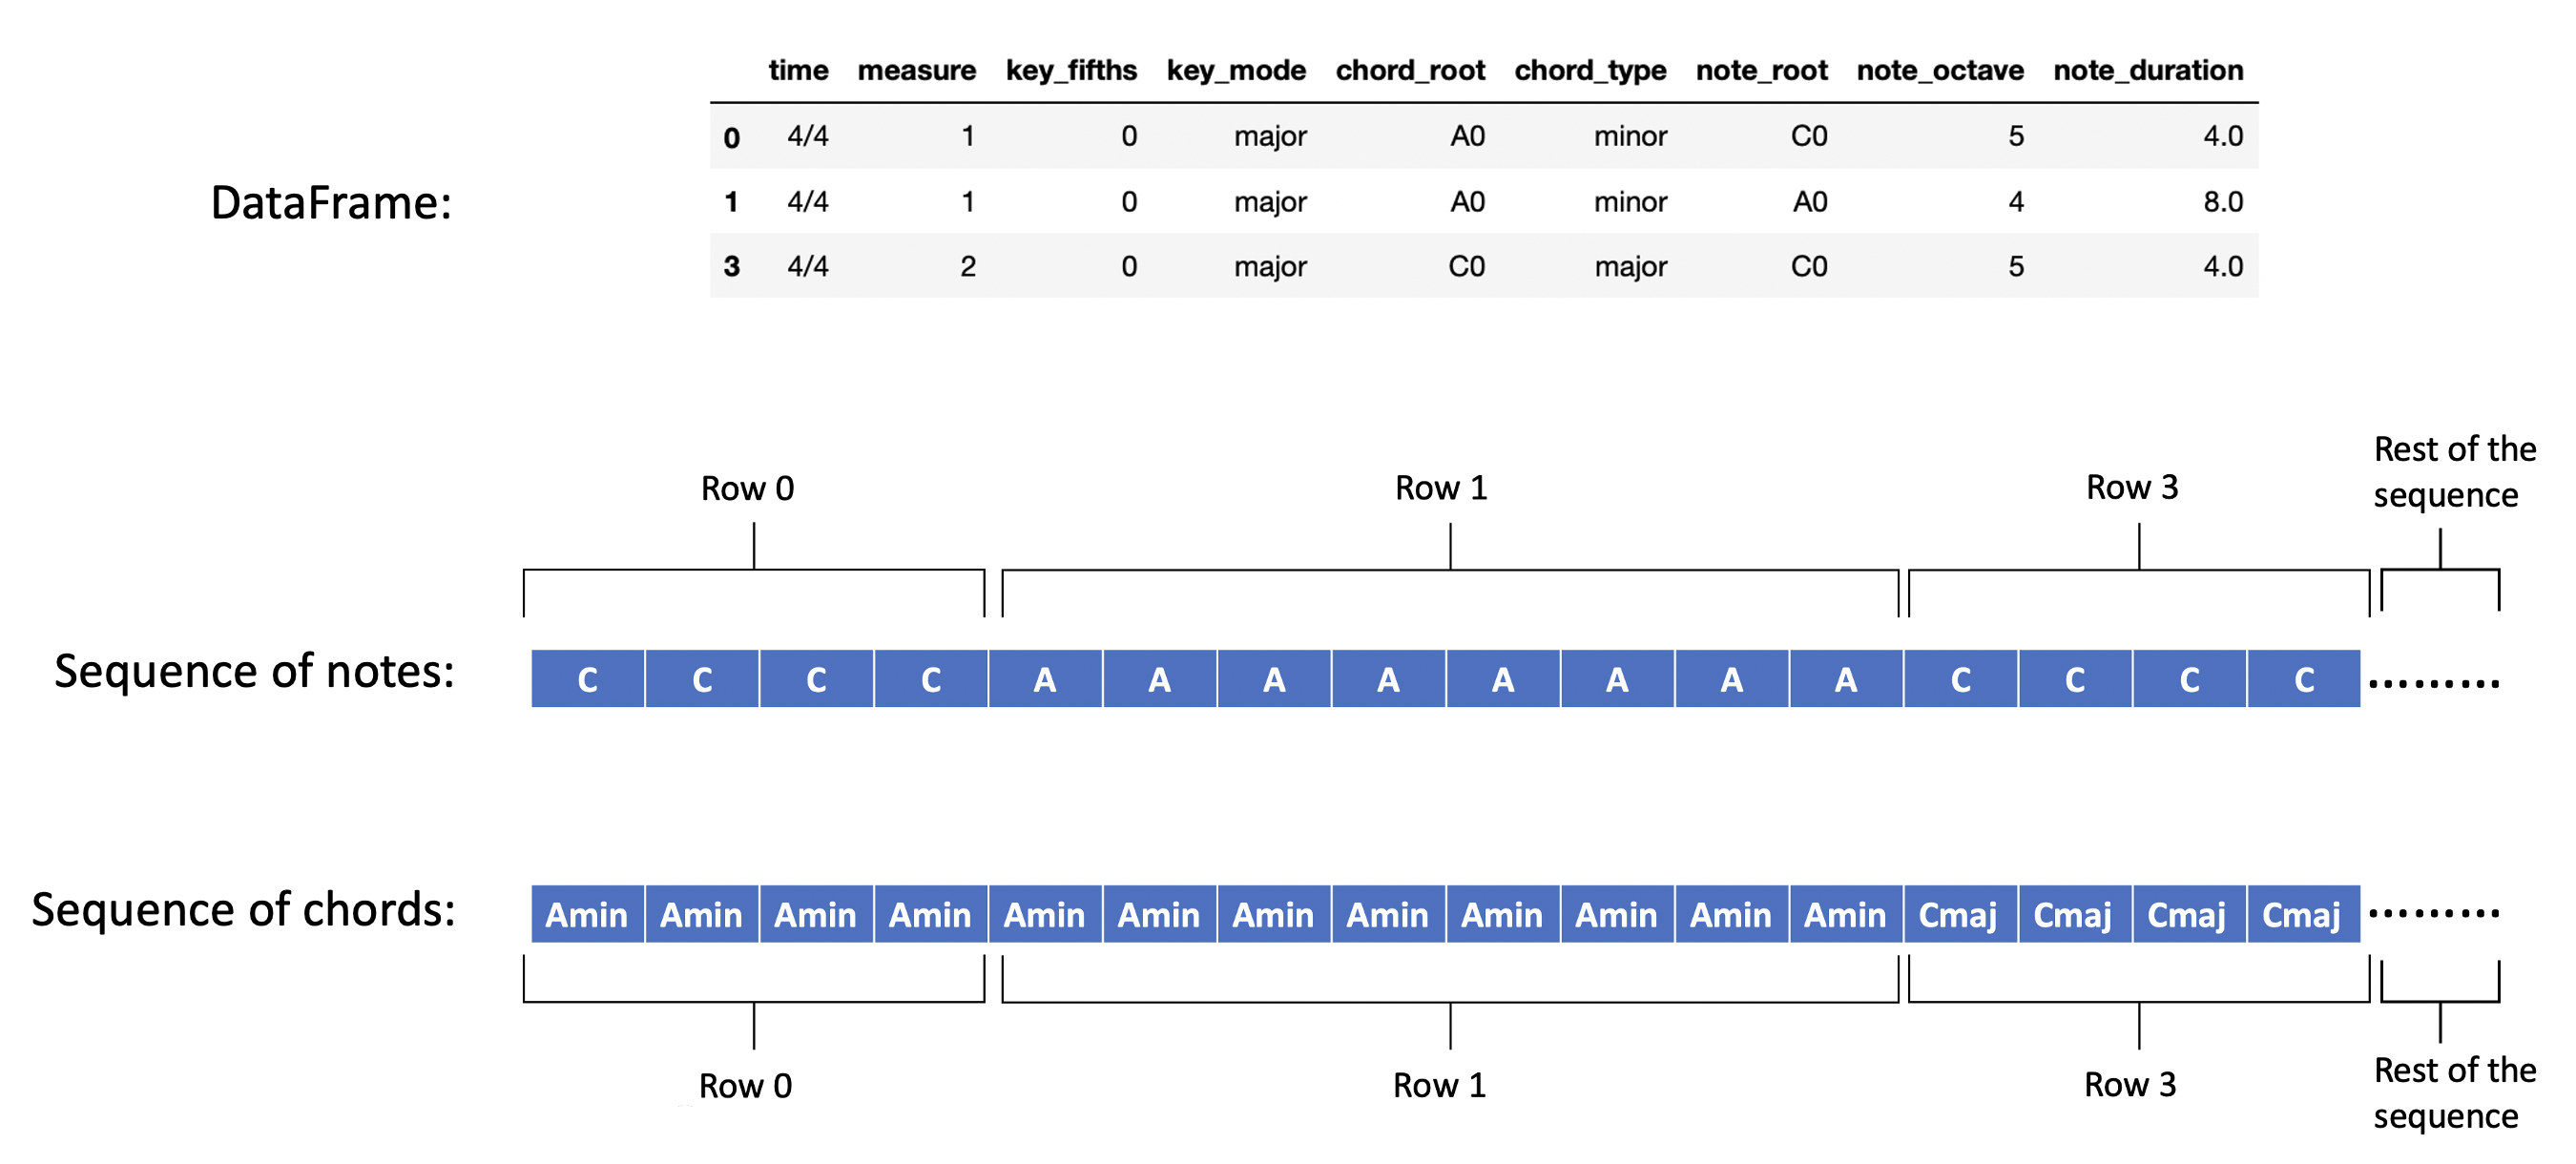
\includegraphics[width=0.4\columnwidth]{Figures/Transformer}
    \decoRule
    \caption{The architecture of a transformer from \cite{Transformers}}
    \label{fig:Transformer}
\end{figure}

The structure of a transformer is shown in \autoref{fig:Transformer}.
The masked multi-head attention block is particularly useful for our use case as it allows for the pre specification of output chords.
Therefore, if a user were to particularly like a certain chord or set of chords it would be possible to lock those in place and generate others around it.

\subsubsection{Possible Implementation}
As, to our knowledge, no implementations of a transformer exist to solve this problem, we now outline how this could be achieved.
Transformers require a symbol picked from a finite set. 
In our case these input symbols would correspond to the note played on each submeasure.
This results in the input data format discussed in \autoref{Transformer format for training}.
The set of output symbols would then consist of the set of possible chords and there would be an output of one chord per submeasure resulting in the corresponding chord data format.
The structure of the transformer can be that used in \cite{Transformers}.
In order to train the model the Adam optimiser, \cite{Adam}, can be used and dropout can be used for regularisation.
Given its success in natural language processing we hypothesise that results from a transformer on this problem would be promising.

\section{Our Model}
\label{Our Model}
We propose the use of a conditional GAN to learn the association between melodies and chords.
It is well demonstrated that a GAN is capable of generating high quality imitations of real data and as a non-deterministic model it fits the criterial outlined in \autoref{sec:MVPRequirements}.
The Discriminator consists of a number of LSTM layers followed by a linear output layer.
The Generator consists of a linear layer followed by a number of LSTM layers and then by another linear layer.
% The Binary Cross Entropy loss is used to determine the Discriminator loss for each example. This is averaged across every measure and then between real and generated examples
\subsection{Components}

\paragraph{Generator}
In essence the Generator functions as a non-deterministic translator, from a sequence of melody vectors to a sequence of chord vectors, and thus models from the NLP space would function appropriately.
Since the LSTM, a common model used in NLP, performed best in \autoref{sec:Evaluation} and is strongly affected by the temporal relationship between inputs, we chose to use it in our Generator.
It takes as input a tensor of dimensions $(b,n,12+l)$ where $b$ is the batch size, $n$ is the number of measures in the song and $l$ is the length of the noise vector.
Each batch is treated independently and identically, so we will proceed discussing the treatment of the 2nd and 3rd dimensions, and it can be assumed this is repeated $b$ times.
Thus, we effectively input a tensor of dimensions $(n,12+l)$ into the first layer of the Generator.
We input the vectors into a linear layer followed by a ReLU activation function. 
These are followed by $k$ layers of bidirection LSTMs.
In the first layer each pair of LSTM cells, one for the forward direction and one for the reverse direction, takes an input vector of length 37, representing a melody vector concatenated with a chord vector and outputs a vector of length $h$ corresponding to the size of the hidden layers.
The LSTM cells in the subsequent $k-1$ layers have both input and output sizes of $h$.
The output of the final LSTM layer is fed into a final linear layer which takes input of size $h$ and outputs a vector of length 25, representing the chords.
This is then passed through a softmax layer which gives the probability that each chord is played at each point in time.

\begin{figure}
    \centering
    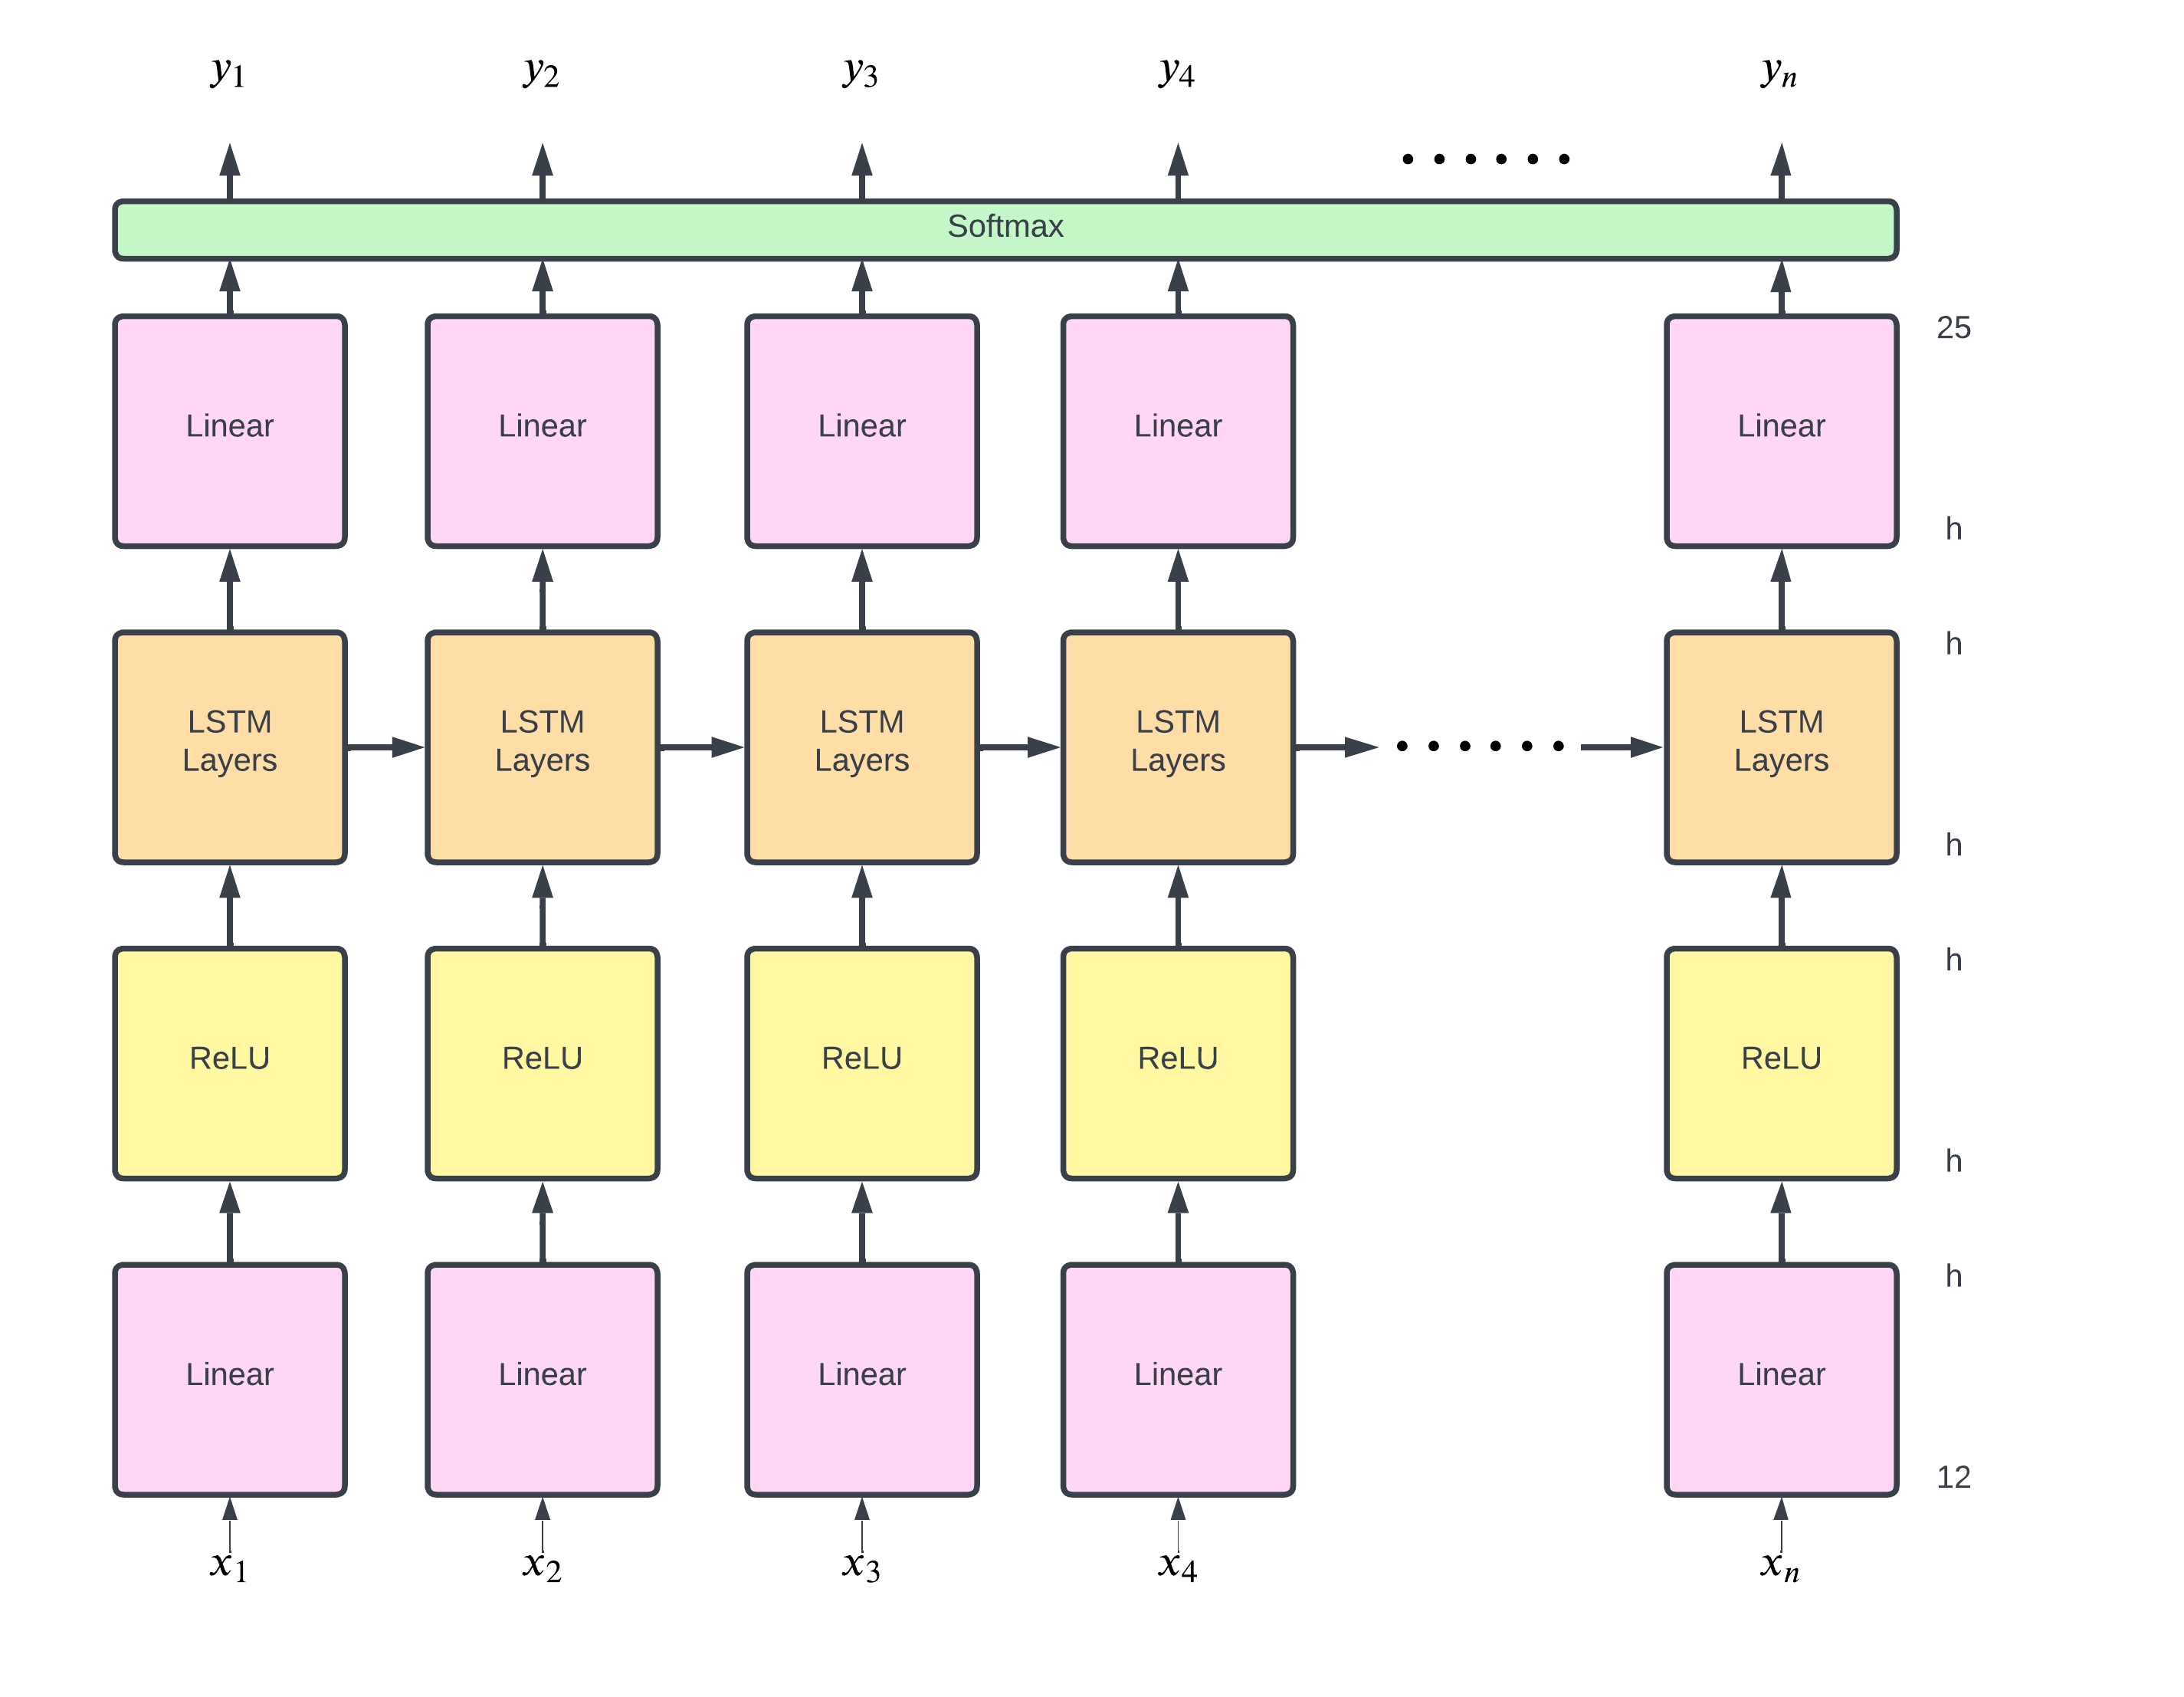
\includegraphics[width=0.8\columnwidth]{Figures/Generator}
    \decoRule
    \caption{The architecture of our Generator}
    \label{fig:Generator}
\end{figure}

\paragraph{Discriminator}
The Discriminator is fundamentally a binary sequence classifier.
It takes as input a tensor of dimensions $(b,n,37)$ where $b$ is the batch size and $n$ is the number of measures in the song.
Each batch is treated independently and identically, so we will proceed discussing the treatment of the 2nd and 3rd dimensions, and it can be assumed this is repeated $b$ times.
Thus, we effectively input a tensor of dimensions $(n,37)$ into the first layer of the Discriminator.
The first $k$ layers of the Discriminator are bidirectional LSTMs. 
These function much like they do in the Generator.
The fully connected layer takes and input of size $2 \times n \times h$ and outputs a vector of size 1.
The output is passed through a sigmoid activation function thus converting it to represent the probability that the input melody sequence, chord sequence pair was from a real song.

\begin{figure}
    \centering
    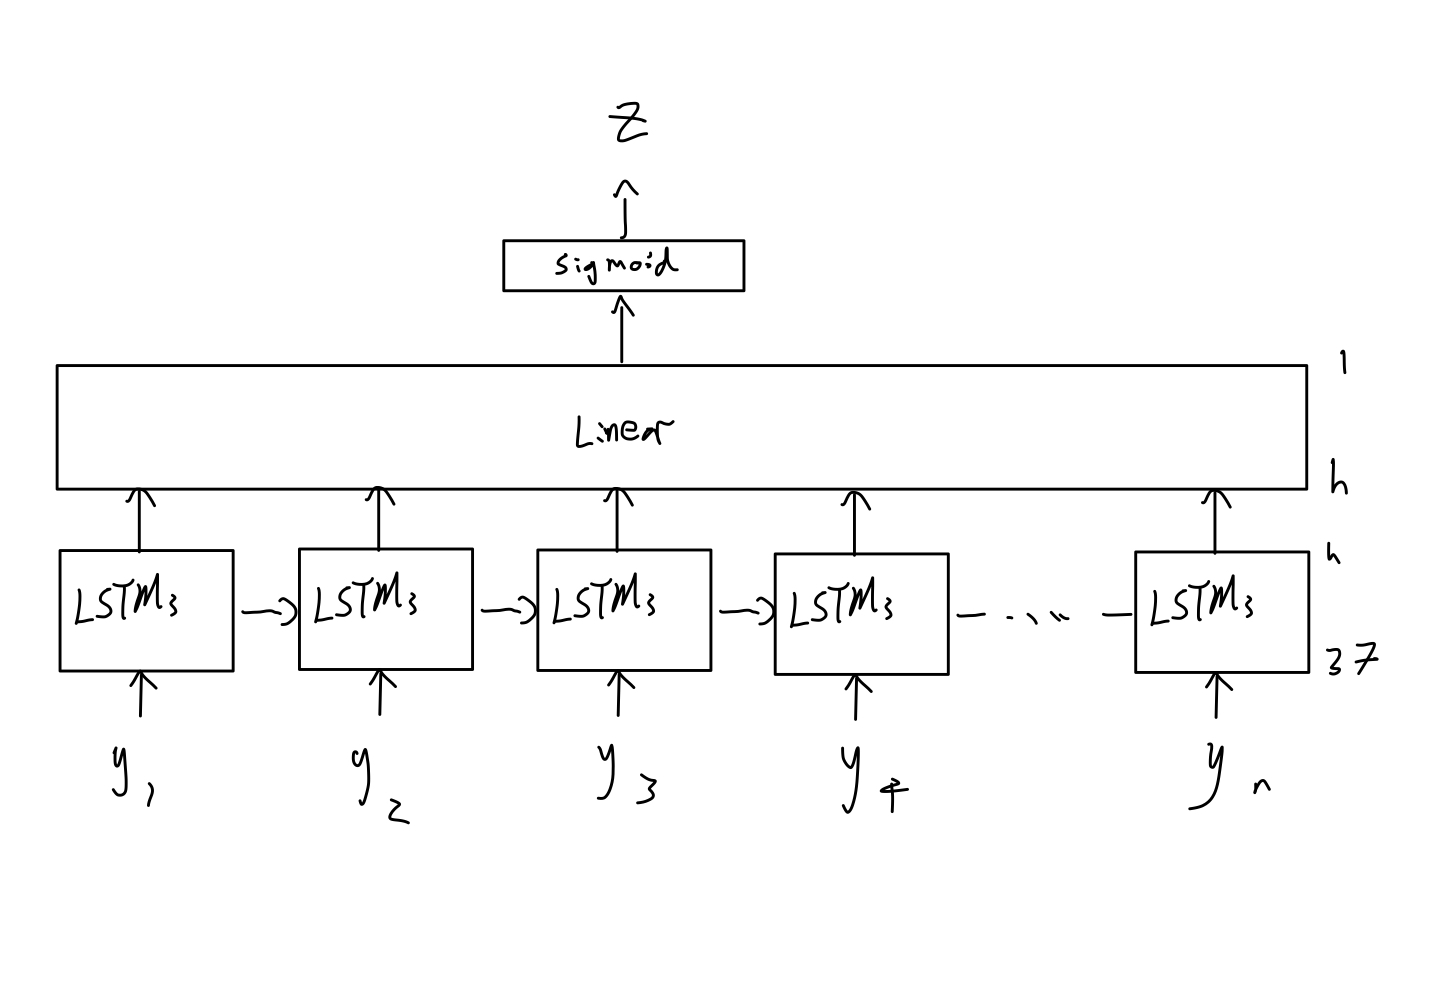
\includegraphics[width=0.8\columnwidth]{Figures/Discriminator}
    \decoRule
    \caption{The architecture of our Discriminator}
    \label{fig:Discriminator}
\end{figure}


\subsection{Model Functionality}

As proof of concept for the design we developed a command line based interface for the model such that it was easy to train, vary parameters and test. 
In production the user would be able to utilise a subset of this interface, such as the option to generate accompaniment and have it played back, through a graphical user interface.
The options available in the interface are shown in \autoref{tab:parameters}

\begin{table}
    \caption{The parameters of the command line interface for the model}
    \label{tab:parameters}
    \centering
    \begin{tabular}{l l l p{0.5\linewidth}}
    \toprule
    \tabhead{Parameter} & \tabhead{Options} & \tabhead{Default} & \tabhead{Description} \\
    \midrule
    \code{-input\_size} & \code{[input\_size]} & $12$ & The size of the input vector to the discriminator representing the melody  \\
    \code{-output\_size} & \code{[output\_size]} & $25$ & The size of the output vector representing the chord played in each measure \\
    \code{-h\_size} & \code{[h\_size]} & $128$ & The size of the hidden layers in the LSTM layers \\
    \code{-n\_layers} & \code{[n\_layers]} & $2$ & The number of LSTM layers in the generator and discriminator \\
    \code{-noise\_size} & \code{[noise\_size]} & $12$ & The size of the noise vector concatenated with the input vector to the generator \\
    \code{-max\_seqlen} & \code{[max\_seqlen]} & $200$ & The maximum length of song in measures used in training \\
    \code{-src\_data} & \code{[src\_data]} &  & The default path to the training data \\
    \code{-batch\_size} & \code{[batch\_size]} & $10$ & The size of the batches used in the stochastic gradient descent algorithm \\
    \code{-epochs} & \code{[epochs]} & $100$ & The number of epochs used in training \\
    \code{-printevery} & \code{[printevery]} & $10$ & The number of epochs between printing an example during training \\
    \code{-load} & & False & Whether to load a model in or not \\
    \code{-load\_dir} & \code{[load\_dir]} &  & The path to the folder containing pretrained models \\
    \code{-model\_num} & \code{[model\_num]} & $1$ & The number of the model to be loaded in \\
    \code{-save} & & False & Whether to save the model after training \\
    \code{-save\_dir} & \code{[save\_dir]} &  & The path to the save directory \\
    \code{-playback} & & False & Whether to play an example of generated music at the end of training \\
    \bottomrule \\
\end{tabular}
\end{table}
 
\paragraph{DataLoader} 
We created a MusicDataset class inheriting from a PyTorch Dataset to load in the data in an useable form.
Since our model takes a fixed sequence length and not all songs are of equal length we zero-pad all songs such that their length is equal to that of the longest song.
The chords are padded with vectors representing a rest.

\section{Training}

\begin{figure}
    \centering
    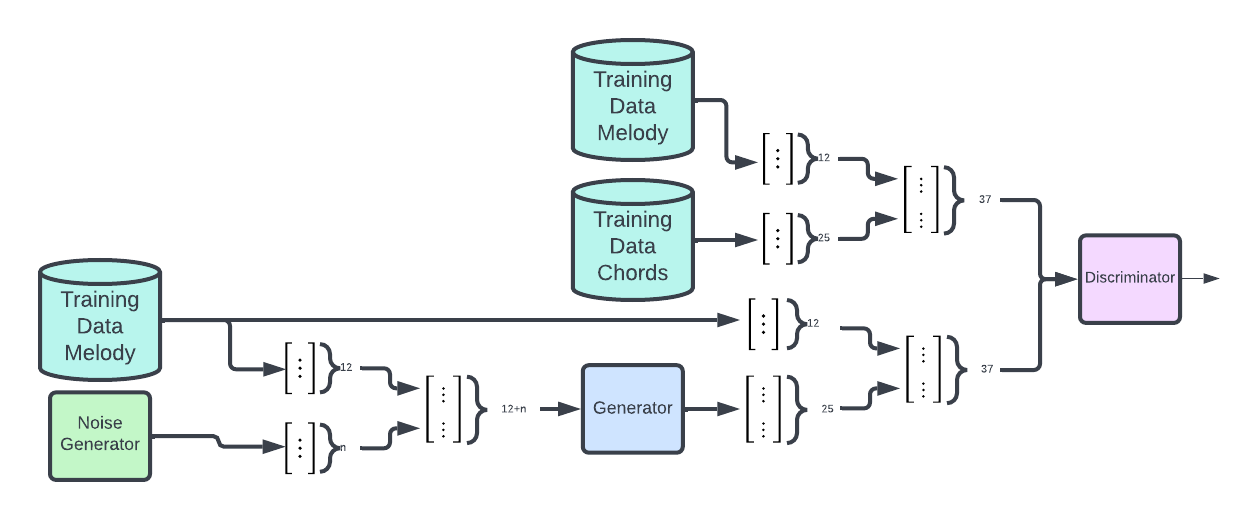
\includegraphics[width=0.8\columnwidth]{Figures/GAN}
    \decoRule
    \caption{The training of the model}
    \label{fig:ModelTraining}
\end{figure}

\paragraph{Loss}
A loss function is used to gain a measure of how different the output of the model is from the desired output.
For best results a loss function is often coupled with the activation function of the linear layers.
An example of this coupling is the sigmoid activation function and the binary cross entropy. %\textbf{EXPAND ON THIS}
As we are using a GAN we use the Binary Cross Entropy or BCE as our loss function for the Discriminator as we are dealing with a binary problem, is the input real or generated?
The Discriminator loss is averaged across its performance between real and generated examples.
For the Generator we use the complement of the Discriminator loss on generated examples.
The BCE loss can be calculated as in \autoref{eq:BCELoss}.
\begin{equation}
    \label{eq:BCELoss}
    \frac{1}{N} \sum_{i=1}^N log(p(y_i))
\end{equation}
    which for the discriminator takes the form
\begin{equation}
    \frac{1}{N} \sum_{i=1}^N log(D(conc(x_i,z_i))) + log(1-D(conc(G(z_i),z_i)))
\end{equation}
    where $x_i$ are the real examples, $z_i$ are the melodies and the $conc$ function concatenates the two vector arguments.
    The loss is the sum of the loss of the discriminator on real data and generated data.
    The generator loss is
\begin{equation}
    -\frac{1}{N} \sum_{i=1}^N log(1-D(conc(G(z_i),z_i)))
\end{equation}
    which results in trying to maximise the loss of the discriminator on generated data.
    This is equivalent to finding the discriminator loss on generated data when labelled as real which is the method we use in our implementation.

    
\paragraph{Optimiser}
An optimiser is used to determine the changes of model parameters that need to be made to minimise the loss of a model.
Optimisers usually involve the use of the gradient of the model with respect to different parameters.
The standard tool to find the gradients is the backpropagation algorithm 
which is very easy to use with PyTorch.
Gradient descent is an example of a basic optimiser.
We used the Adam optimiser \cite{Adam} which is recommended in the Stanford \href{https://cs231n.github.io/}{CS231n: Convolutional Neural Networks for Visual Recognition}\footnote{https://cs231n.github.io/} as the default optimiser.




\subsection{Avoiding Overfitting}
A common problem in machine learning is overfitting. This is where a dataset is modelled to such a precision that noise in the dataset is learned.
This results in the model missing the overarching distribution of the data and thus cannot extend to other data.
There is a number of techniques to avoid overfitting.
Dropout is where neurons are ignored with a given probability on any given pass. 
This is equivalent to training a number of different neural networks which all overfit in different ways thus on average the overfitting will cancel out.
Another technique to reducing overfitting specific to GANs is to use the Wasserstein loss function rather than the binary cross entropy. 
This was first proposed in \cite{Wasserstein} and uses the difference of the output from the discriminator on real and generated data as the discriminator loss and uses the output of the discriminator on generated data as the generator loss.
This means that gradients do not vanish as fast, however, the output of the discriminator no longer represents the probability of the input being true.
Another technique is reducing number of LSTM layers. 
This reduces the complexity of the model and thus makes it harder to train it to overfit onto noise.

\subsection{Issues}
Training is conducted in batches of a given size.
It is unlikely that the size of the dataset is divisible by the batch size, so the final batch is likely to be shorter than the others.
This initially caused problems, however, we were able to set the dimensions of relevant objects, such as the input noise to the generator, to be relative to the current batch size rather than the usual batch size thus solving the problem.
Softmaxing of outputs of generator
Device management

\subsection{Testing}
The Model can be tested using the test set as this will reveal any overfitting from training. 
We can evaluate the model as stated in \autoref{sec:Evaluation} using the accuracy of the model across the test set.
Another way we can evaluate the model to get a better sense of where and how the model is going wrong is by using a confusion matrix.
We enumerate the generated chords and the true chords. 
For each melody we add one to the element in the (generated chord, true chord) coordinate. 
Thus, an ideal output would be a diagonal matrix such that the generated chord was always the same as the true chord, however, this would also suggest overfitting.
An example of a confusion matrix is shown in \autoref{fig:confusion_ideal}
Another form of testing that could be performed is a subjective study like those in \cite{MySong} and \cite{BLSTM}.
Ideally the studies would be carried out as similarly as possible to the others such that the models they are testing can be reliably compared.

\begin{figure}
    \centering
    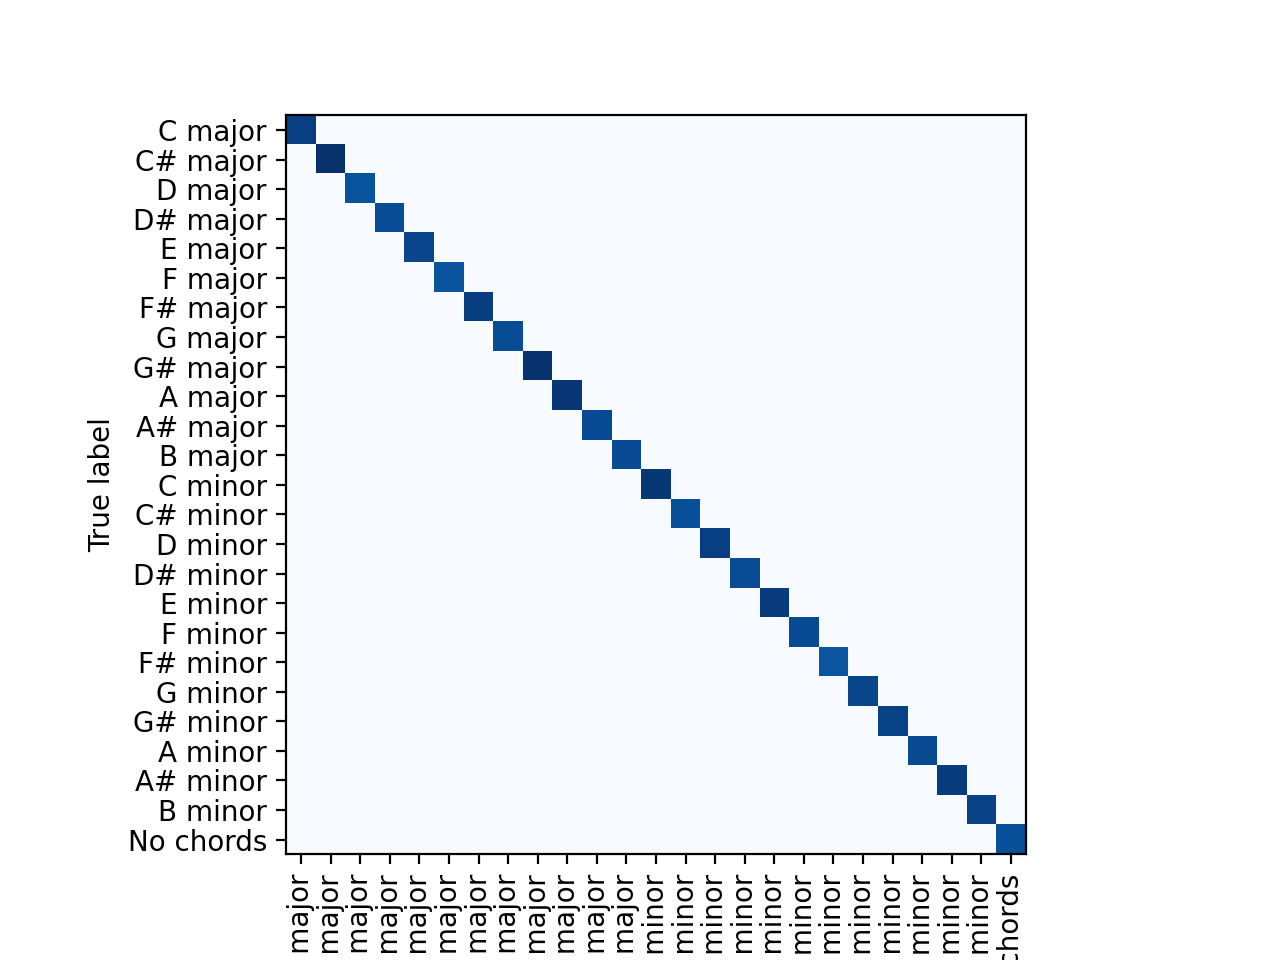
\includegraphics[width=0.4\columnwidth]{Figures/confusion_ideal}
    \decoRule
    \caption{An ideal confusion matrix}
    \label{fig:confusion_ideal}
\end{figure}

\section{Results}
Unfortunately due to implementation difficulties followed by the sudden death of the machine we were using to train the model we were unable to obtain any valid results.
While the machine was still running we conducted some preliminary training attempts where convergence of the GAN illuded us.
The discriminator quickly learned to distinguish between the real and generated chords and the generator was never able to improve sufficiently to counter this.
The loss of the models can be seen in \autoref{fig:ModelLoss}.
It was noticed that the generator converged to predict the same chord on every output. 
This is likely due to a combination of overfitting of the linear output layer in the generator and the vanishing of gradients as the discriminator loss was effectively zero.
A confusion matrix of these results can be seen in \autoref{fig:confusion_real}. As mentioned earlier in the report, the code for this project can be found \href{https://github.com/edsgunn/TerrenceInABox}{here}\footnote{https://github.com/edsgunn/TerrenceInABox}.
\begin{figure}
    \centering
    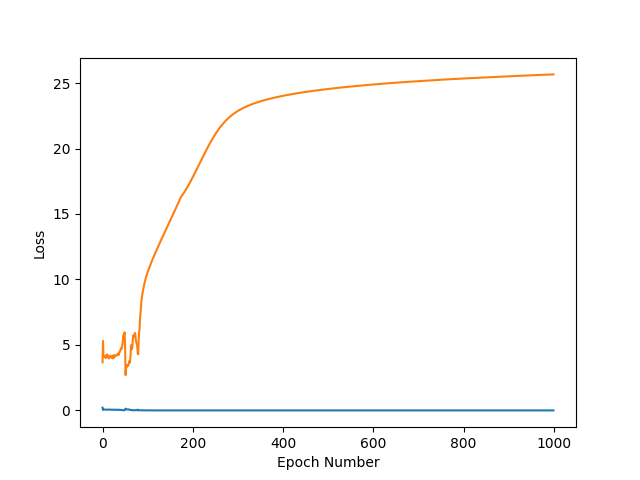
\includegraphics[width=0.4\columnwidth]{Figures/ModelLoss}
    \decoRule
    \caption{The loss of the Generator and Discriminator, blue and orange respectively}
    \label{fig:ModelLoss}
\end{figure}

\begin{figure}
    \centering
    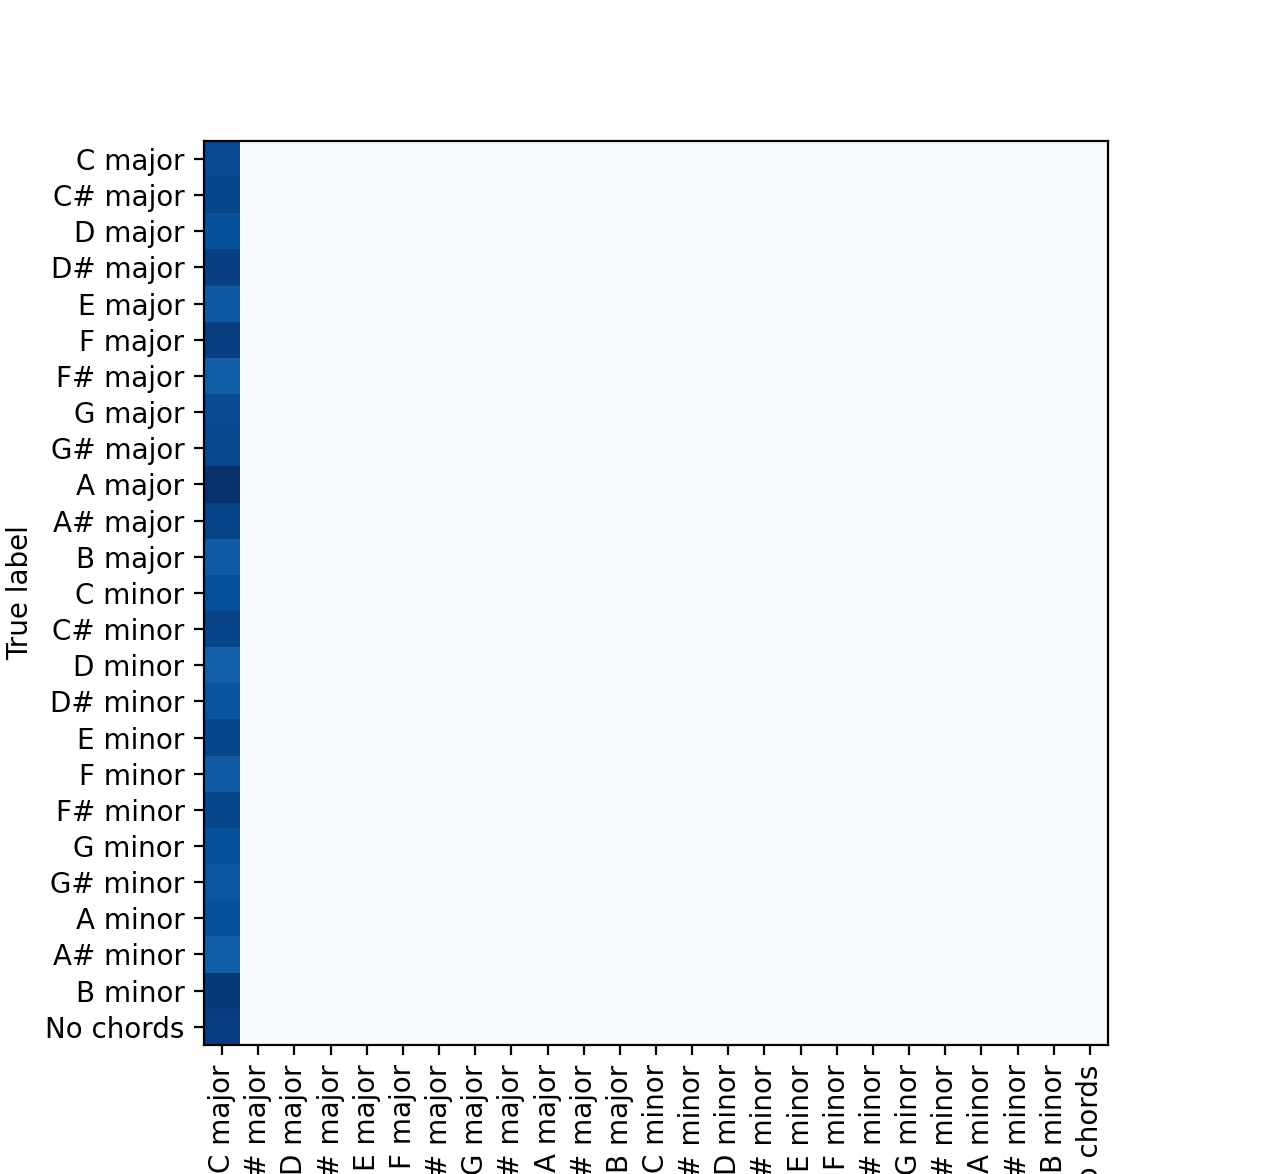
\includegraphics[width=0.4\columnwidth]{Figures/confusion_real}
    \decoRule
    \caption{A confusion matrix of the chords outputted from the model}
    \label{fig:confusion_real}
\end{figure}